\numberwithin{equation}{chapter}
\numberwithin{equation}{section}
\baselineskip=8mm
\chapter{การวิเคราะห์และการออกแบบระบบ}

% \renewcommand{\thesubsection}{\thechapter.\arabic{subsection}}
\renewcommand{\thesubsection}{\arabic{subsection}.}
\renewcommand{\theequation}{\thesection.\arabic{equation}}
\renewcommand{\thesection}{}


\section{การออกแบบระบบ}

\section{Use Case Diagram}

\section{Use Case Description}

\section{Class Diagram}

\section{Class Description}

\section{Entity-Relationship Diagram}

\begin{figure}[h!]
   \centering
   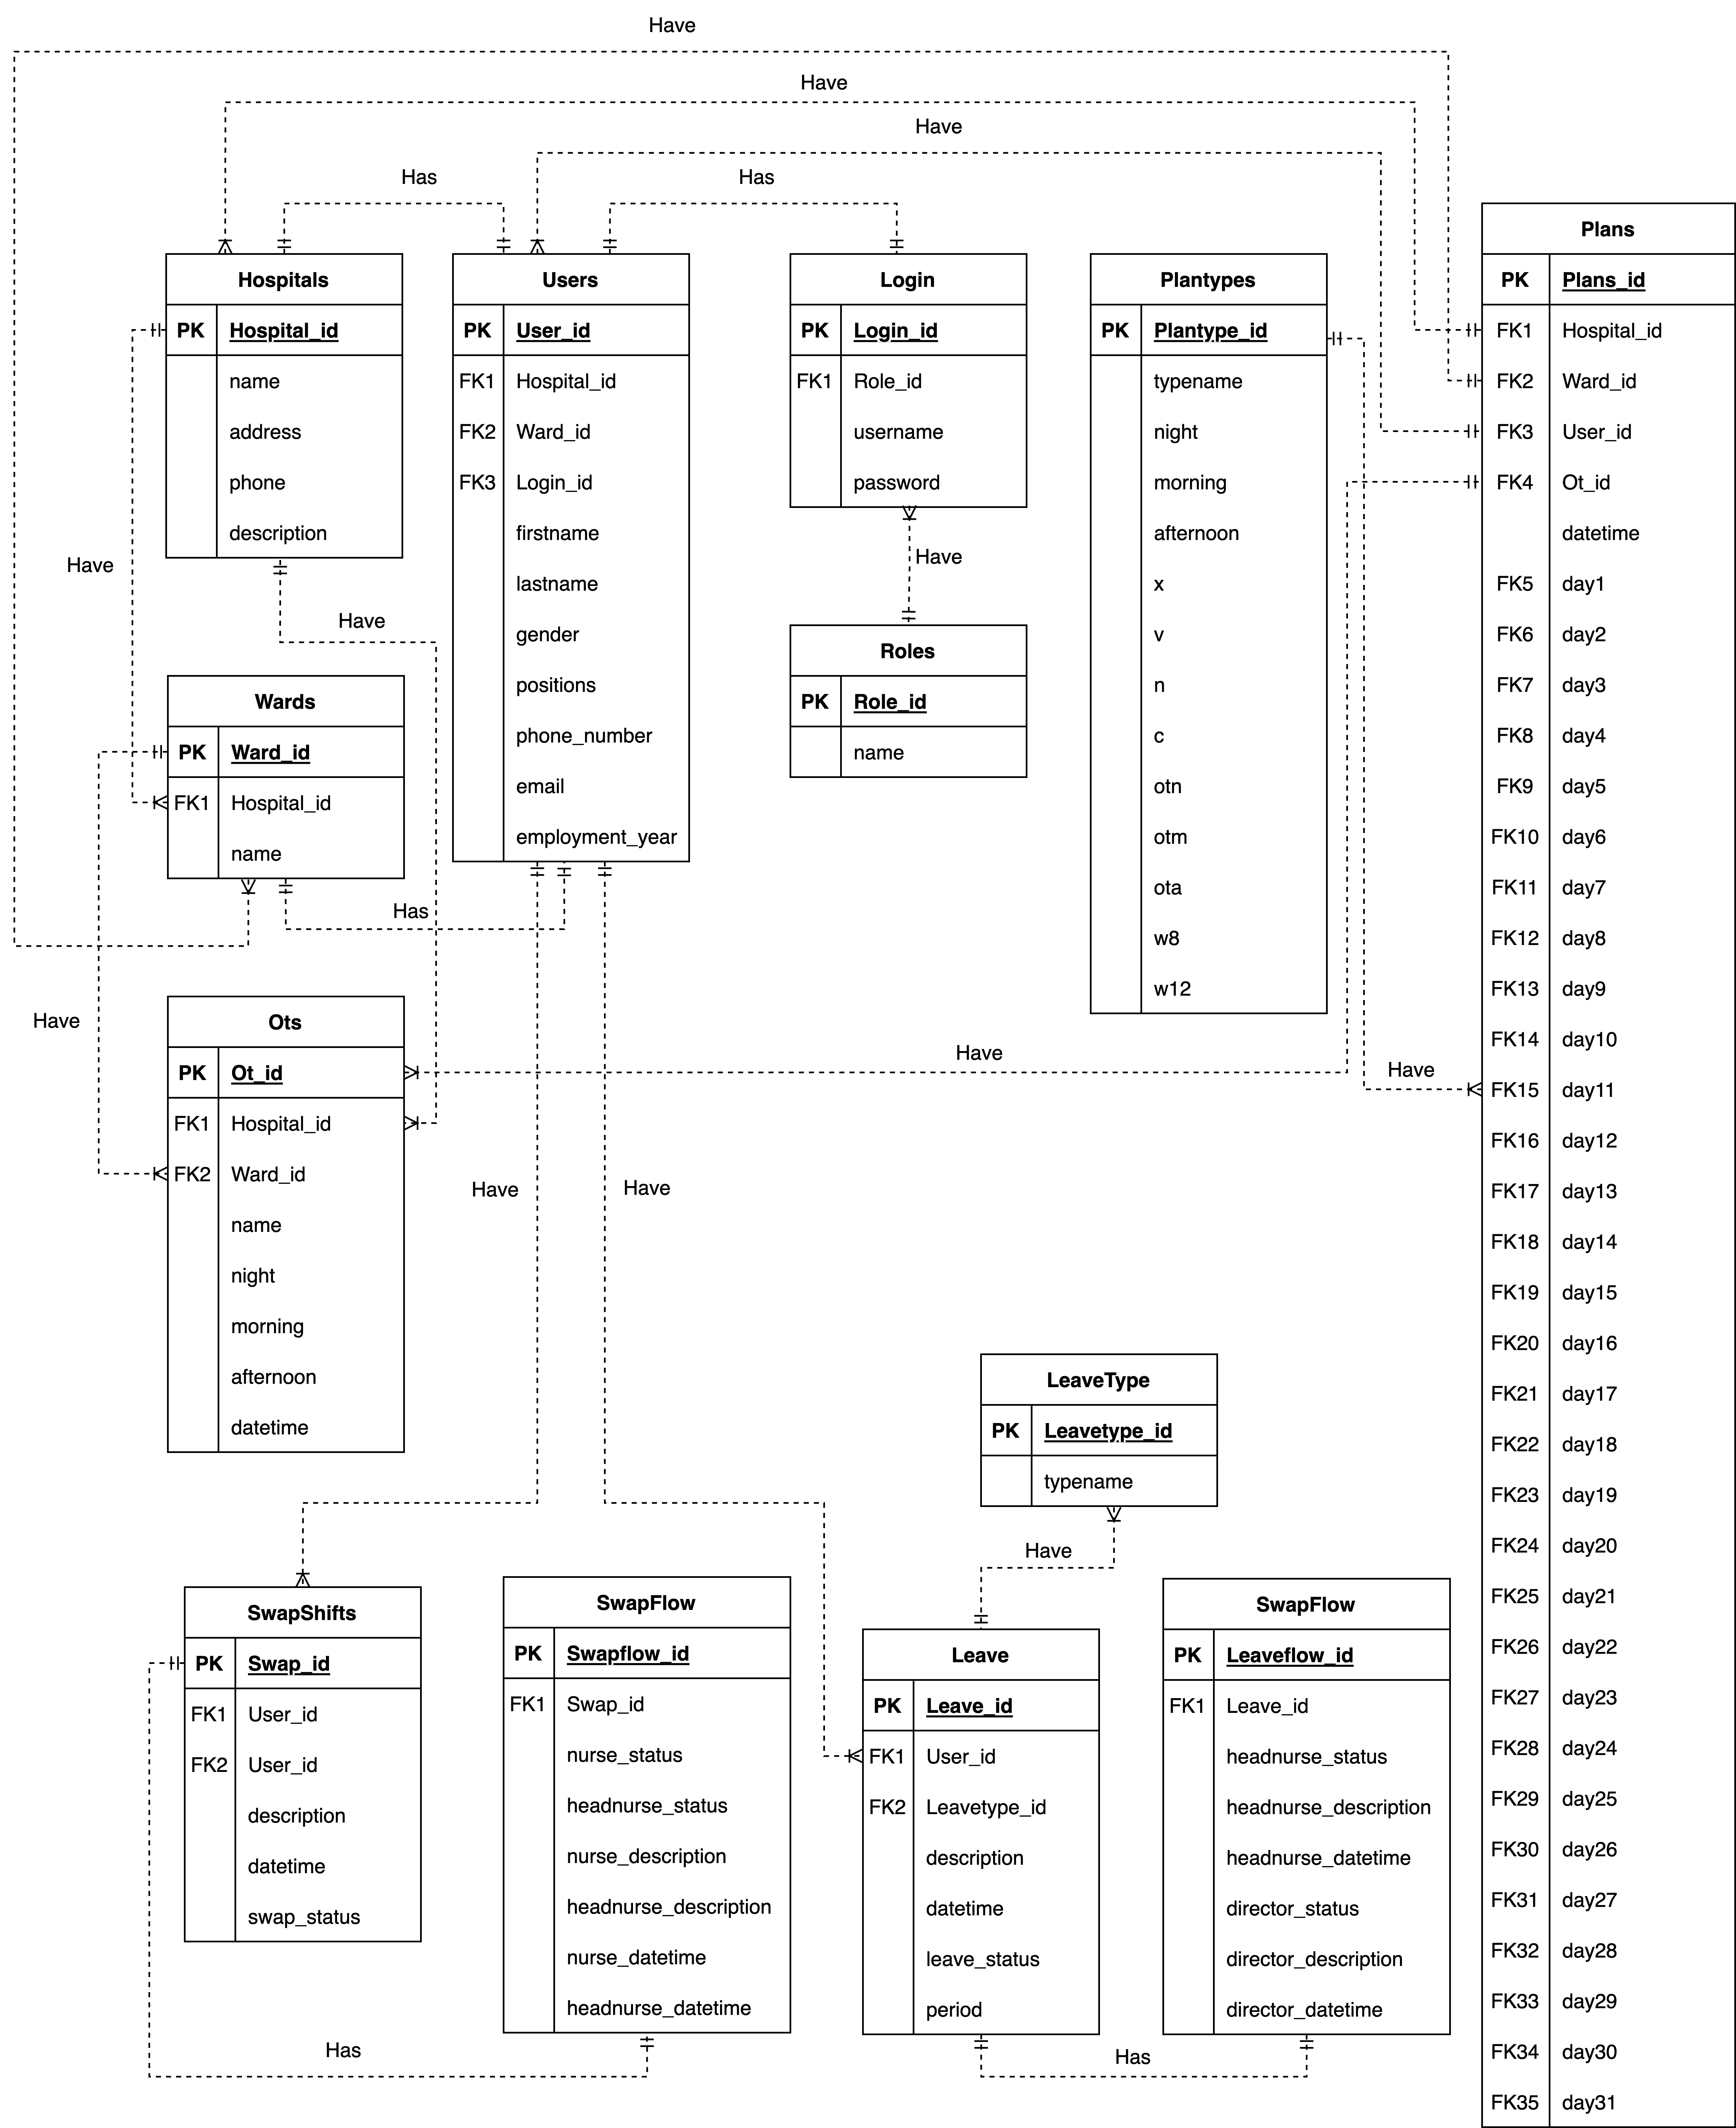
\includegraphics[width=1\textwidth]{ER.png}
   \caption{Entity-Relationship Diagram}
\end{figure}

\section{Entity-Relationship Description}

\section{การออกแบบหน้าจอแสดงผล}

\subsection{User 1}

\subsection{User 2}

\subsection{User 3}

\subsection{User 4}

\subsection{User 5}

